\documentclass{article}
\usepackage[utf8]{inputenc}
\usepackage{amsmath}
\usepackage{amssymb}
\usepackage{amsfonts}
\usepackage{amsthm}
\usepackage{parskip}
\usepackage{listings}
\usepackage{pgfplots}
\usepackage{pgfkeys}
\pgfplotsset{compat=1.17}
\usepackage{tikz}
\usetikzlibrary{chains,shadows.blur,shapes.geometric}
\usetikzlibrary{automata,positioning}
\usetikzlibrary{trees}


\title{HW2}
\author{Asier Garcia Ruiz}

\begin{document}
\maketitle

\section*{Question 1.}
\subsection*{a)}
\begin{verbatim}
    Instructions:           Cost:
    1. lshi 2, i, t1        1
    2. add b, t1, t2        2
    3. lw t2, t3            7
    4. lshi 2, i, t1        1
    5. add a, t4, t5        2
    6. muli 3, tj, t6       4
    7. lshi 2, t6, t7       1
    8. add a, t7, t8        2
    9. lw t8, t9            7
    10. sw t9, t5           4
\end{verbatim}

Total cost is 31.

\subsection*{b)}
\begin{figure}[h]
    \centering
    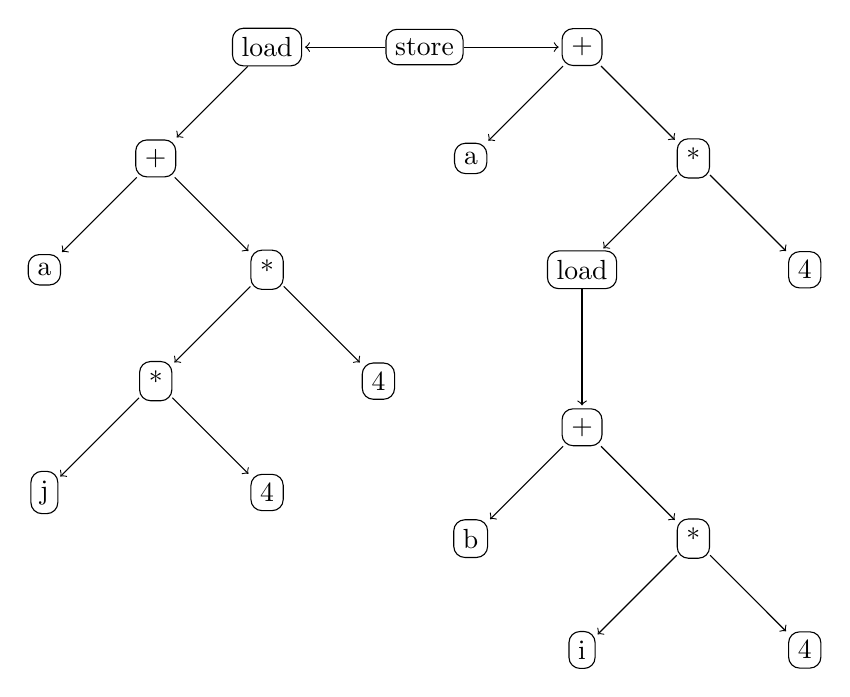
\begin{tikzpicture}[shorten >=1pt,node distance=2cm,on grid,auto, box/.style = {draw,rounded corners,fill=white, align=center}]
        \node[box] (store1)   {store};
        \node[box] (load1) [left of=store1]  {load};
        \node[box] (plus1) [right of=store1]  {+};
        \node[box] (a1) [below left of=plus1]  {a};
        \node[box] (mult1) [below right of=plus1]  {*};
        \node[box] (load2) [below left of=mult1]  {load};
        \node[box] (41) [below right of=mult1]  {4};
        \node[box] (plus2) [below of=load2]  {+};
        \node[box] (b) [below left of=plus2]  {b};
        \node[box] (mult2) [below right of=plus2]  {*};
        \node[box] (i) [below left of=mult2]  {i};
        \node[box] (42) [below right of=mult2]  {4};
        \node[box] (plus3) [below left of=load1]  {+};
        \node[box] (a2) [below left of=plus3]  {a};
        \node[box] (mult3) [below right of=plus3]  {*};
        \node[box] (mult4) [below left of=mult3]  {*};
        \node[box] (43) [below right of=mult3]  {4};
        \node[box] (j) [below left of=mult4]  {j};
        \node[box] (3) [below right of=mult4]  {4};

        \path[->]
        (store1)
        edge node {} (load1)
        edge node {} (plus1)
        (plus1)
        edge node {} (a1)
        edge node {} (mult1)
        (mult1)
        edge node {} (load2)
        edge node {} (41)
        (load2)
        edge node {} (plus2)
        (plus2)
        edge node {} (b)
        edge node {} (mult2)
        (mult2)
        edge node {} (i)
        edge node {} (42)
        (load1)
        edge node {} (plus3)
        (plus3)
        edge node {} (a2)
        edge node {} (mult3)
        (mult3)
        edge node {} (mult4)
        edge node {} (43)
        (mult4)
        edge node {} (j)
        edge node {} (3)
        ;
    \end{tikzpicture}
\end{figure}
\newpage

\subsection*{c)}
\begin{verbatim}
    lwo i, b, t1
    lshi 2, t0, t1
    muli 3, j, t2
    lshi 2, t2, t3
    mmc a, t3, t1
\end{verbatim}
Total cost is 25.

\subsection*{d)}
\begin{verbatim}
    lwo i, b, t0        7
    lshi 2, t0, t1      1
    add t1, a, t2       2
    muli 3, j, t3       4
    lwo t3, a, t4       7
    sw t4, t2           3
\end{verbatim}

Total cost is 25.

\section*{Question 2}
\subsection*{a)}

We have that
\begin{align*}
    n   & = \{3\pm \}, \\
    acc & = [2+, 10+], \\
    ctr & = [3+, 9+],  \\
    con & = [5+, 5+],  \\
\end{align*}

\subsection*{b)}

\begin{figure}[h]
    \centering
    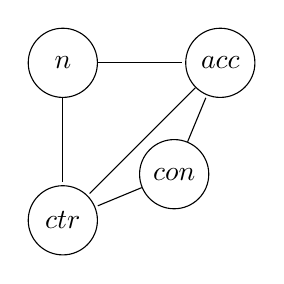
\begin{tikzpicture}[shorten >=1pt,node distance=2cm, on grid, auto]
        \node[state] (n)   {$n$};
        \node[state] (acc) [right=of n] {$acc$};
        \node[state] (ctr) [below=of n] {$ctr$};
        \node[state] (con) [below right=of n] {$con$};
        \path[-]
        (n)
        edge node {} (ctr)
        edge node {} (acc)
        (con)
        edge node {} (ctr)
        edge node {} (acc)
        (acc)
        edge node {} (ctr);
    \end{tikzpicture}
\end{figure}

\subsection*{c)}
From the interference graph we know that the minimum required registers for spill-free execution is 3.
We can write the program as

\begin{verbatim}
    1. start:
    2.  r1 := 1
    3.  r2 := r3
    4. loop:
    5.  r3 := r2 <= 1
    6.  br r3, done
    7.  r1 := r1 * r2
    8.  r2 := r2 - 1
    9.  jmp loop
    10. done:
\end{verbatim}

\section*{Question 3.}
\subsection*{a)}
We can use the following registers

\begin{verbatim}
    1. r1 := X + i
    2. r2 := *r1
    3. *Z := r2
    4. r1 := r1 + 2
    5. r2 := *N
    6. r1 := r2 + r1
\end{verbatim}

This uses only two registers $r_1, r_2$. The new dependence graph is

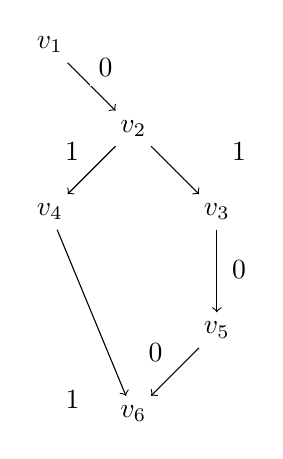
\begin{tikzpicture}[main/.style = {draw, circle}, node distance=1.5cm]
    \node[] (1) {$v_1$};
    \node[] (2) [below right of=1] {$v_2$};
    \draw [->] (1) -- (2) node [yshift=22pt, xshift=-10pt, fill=white] {0};

    \node[] (3) [below right of=2] {$v_3$};
    \draw [->] (2) -- (3) node [yshift=22pt, xshift=8pt, fill=white] {1};

    \node[] (4) [below left of=2] {$v_4$};
    \draw [->] (2) -- (4) node [yshift=22pt, xshift=8pt, fill=white] {1};

    \node[] (5) [below of=3]{$v_5$};
    \draw [->] (3) -- (5) node [yshift=22pt, xshift=8pt, fill=white] {0};

    \node[] (6) [below left of=5] {$v_6$};
    \draw [->] (5) -- (6) node [yshift=5pt, xshift=-22pt, fill=white] {1};
    \draw [->] (4) -- (6) node [yshift=22pt, xshift=8pt, fill=white] {0};
\end{tikzpicture}

We can schedule the instructions in the order
\begin{align*}
    \text{Clock Cycle}\qquad & \text{Instruction}, \\
    1:\qquad                 & v_1                 \\
    2: \qquad                & v_2                 \\
    3: \qquad                & v_2                 \\
    4:  \qquad               & v_3                 \\
    5:  \qquad               & v_5                 \\
    6:  \qquad               & v_5, v_4            \\
    7:   \qquad              & v_6
\end{align*}
It takes 7 cycles to execute with a scheduling of $\{v_1, v_2, v_3, v_5, v_4, v_6\}$.

The number of registers is 2 and the completion time is 7

\subsection*{b)}
We can schedule the instructions in the order
\begin{align*}
    \text{Clock Cycle}\qquad & \text{Instruction}, \\
    1:\qquad                 & v_1                 \\
    2: \qquad                & v_2                 \\
    3: \qquad                & v_2, v_4            \\
    4:  \qquad               & v_5                 \\
    5:  \qquad               & v_5, v_3            \\
    6:   \qquad              & v_6
\end{align*}
It takes 6 cycles to execute.

Then, we allocate the registers as following
\begin{verbatim}
    1. r1 := X + i
    2. r2 := *r1
    3. *Z := r2
    4. r1 := r1 + 2
    5. r3 := *N
    6. r2 := r3 + r1
\end{verbatim}
This uses 3 registers.

\subsection*{c)}
Using a hybrid approach we can allocate the registers as

\begin{verbatim}
    1. r1 := X + i
    2. r2 := *r1
    3. *Z := r2
    4. r1 := r1 + 2
    5. r2 := *N
    6. r1 := r2 + r1
\end{verbatim}

We can schedule the instructions in the order
\begin{align*}
    \text{Clock Cycle}\qquad & \text{Instruction}, \\
    1:\qquad                 & v_1                 \\
    2: \qquad                & v_2                 \\
    3: \qquad                & v_2                 \\
    4:  \qquad               & v_3                 \\
    5:  \qquad               & v_5                 \\
    6:  \qquad               & v_5, v_4            \\
    7:   \qquad              & v_6
\end{align*}
It takes 7 cycles to execute with a scheduling of $\{v_1, v_2, v_3, v_5, v_4, v_6\}$
\end{document}